\documentclass[12pt, letterpaper, preprint]{aastex}
\usepackage[breaklinks,colorlinks, urlcolor=blue,citecolor=blue,linkcolor=blue]{hyperref}
\usepackage{color}
%%% This file is generated by the Makefile.
\newcommand{\giturl}{\url{https://github.com/changhoonhahn/nonGaussLike}}
\newcommand{\githash}{0cff07b}\newcommand{\gitdate}{2018-01-09}\newcommand{\gitauthor}{ChangHoon Hahn}


% typesetting shih
\linespread{1.08} % close to 10/13 spacing
\setlength{\parindent}{1.08\baselineskip} % Bringhurst
\setlength{\parskip}{0ex}
\let\oldbibliography\thebibliography % killin' me.
\renewcommand{\thebibliography}[1]{%
  \oldbibliography{#1}%
  \setlength{\itemsep}{0pt}%
  \setlength{\parsep}{0pt}%
  \setlength{\parskip}{0pt}%
  \setlength{\bibsep}{0ex}
  \raggedright
}
\setlength{\footnotesep}{0ex} % seriously?

% math shih
\newcommand{\setof}[1]{\left\{{#1}\right\}}
\newcommand{\given}{\,|\,}
\newcommand{\pseudo}{{\mathrm{pseudo}}}
\newcommand{\Var}{\mathrm{Var}}
% text shih
\newcommand{\foreign}[1]{\textsl{#1}}
\newcommand{\etal}{\foreign{et~al.}}
\newcommand{\opcit}{\foreign{Op.~cit.}}
\newcommand{\documentname}{\textsl{Article}}
\newcommand{\equationname}{equation}
\newcommand{\bitem}{\begin{itemize}}
\newcommand{\eitem}{\end{itemize}}
\newcommand{\beq}{\begin{equation}}
\newcommand{\eeq}{\end{equation}}
\newcommand{\todo}[1]{{\bf \textcolor{red}{#1}}}

\newcommand{\patchy}{{\fontshape\scdefault\selectfont patchy}}

\begin{document}\sloppy\sloppypar\frenchspacing 

\title{How I Learned to Stop Worrying and Love The Central Limit Theorem}
\date{\texttt{DRAFT~---~\githash~---~\gitdate~---~NOT READY FOR DISTRIBUTION}}
\author{ChangHoon~Hahn\refstepcounter{footnote}\refstepcounter{footnote}, Florian~Beutler, Manodeep~Sinha, Andreas~Berlind}
\affil{Lawrence Berkeley National Laboratory, 1 Cyclotron Rd, Berkeley CA 94720, USA}
\email{changhoon.hahn@lbl.gov}

\begin{abstract}
    abstract here 
\end{abstract}

\keywords{
methods: statistical
---
galaxies: statistics
---
methods: data analysis
---
cosmological parameters
---
cosmology: observations
---
large-scale structure of universe
}

\section{Introduction}
\begin{itemize}
    \item Talk about the use of Bayesian parameter inference and getting the posterior in LSS cosmology 
    \item Explain the two major assumptions that go into evaluating the likelihood
    \item Emphasize that we are not talking about non-Gaussian contributions to the likelihood
    \item Emphasize the scope of this paper is to address whether one of the assumptions matters for 
        galaxy clustering analyses. 
\end{itemize}

\section{Gaussian Likelihood Assumption}
\begin{itemize}
    \item Depending on Hogg's paper maybe a simple illustration of how the likelihood asumption 
\end{itemize}


\section{Mock Catalogs}
Mock catalogs play a key role in standard cosmological anslyses of LSS 
studies. They're extensively used for testing analysis 
pipelines~\cite[(mock challenege papers)][]{beutler2017}, 
testing the effect of systematics~\citep{hahn2017}, and, most relevantly 
for this paper, for estimating the covariance matrix used in evaluating 
the likelihood for parameter inference~\citep[cite the bunch of other papers][]{beutler2017}.

Maybe a little paragraph about the advantages of covariance matrices from 
mocks versus analytic? 

Our primary goal in this paper is to test the Gaussian likelihood assumption 
in two LSS analyses: the powerspectrum multipole full shape analysis of \cite{beutler2017} 
and group multiplicity function analysis of \cite{sinha2017}. Throughout
the paper we will make extensive use of the mock catalogs used in these 
analyses. Below, in this section, we give a brief description of these mocks. 

\subsection{MultiDark-\patchy~Mock Catalog} 
In their powerspectrum multipole full shape analysis, \cite{beutler2017}
use the MultiDark-\patchy~mock catalogs from \cite{kitaura2016}. 


The dark matter fields for these mocks are generated using approxiate
gravity solvers on a mesh. 


\todo{something about the approximate gravity solver} 
These mock catalogs have been calibrated to high fidelity BigMultiDark 
simulations~\citep{rodriguez-torres2016, klypin2016}

In total \cite{beutler2017} 



%These mock catalogues have been calibrated to an N-body-based reference sample using approximate gravity solvers and analytical–statistical biasing models. The reference catalogue is extracted from one of the BigMultiDark simula- tions (Klypin et al. 2016), which used 38403 particles on a volume of (2.5 h−1 Mpc)3 assuming a  CDM cosmology
%Halo abundance matching is used to reproduce the observed BOSS two- and three-point clustering measurements (Rodrguez- Torres et al. 2016). This technique is applied at different redshift bins to reproduce the BOSS DR12 redshift range. These mock cata- logues are combined into light cones, also accounting for selection effects and masking. In total, we have 2045 mock catalogues avail- able for the NGC and 2048 mock catalogues for the SGC.
\bitem
    \item 2048 mocks for both north and south 
    \item Note that 3 mocks were fixed
\eitem

\subsection{\cite{sinha2017} Mock Catalog}

\subsection{}
${\bf X}_i = [P_0(k)_i,P_2(k)_i,P_4(k)_i]$
${\bf X}_i = \zeta(N)_i$


\section{Likelihood non-Gaussianity}
\subsection{Quantifying the non-Gaussianity}
In \cite{sellentin2017}
One way of quantifying the non-Gaussianity of the likelihood is to 
calculate the divergence between the distribution $p(x)$, which generated
the observable, and $q(x)$ a multivariate Gaussian described by the average
of the mocks and the covariance matrix ${\bf C}$.

Take for instance, the R\'enyi-$\alpha$ divergence between $p(x)$ and $q(x)$ 
\beq
D_{R-\alpha} ( p \parallel q ) = \frac{1}{\alpha -1} \log \int p^\alpha(x) q^{1 -\alpha}(x)\,{\rm d}x. 
\eeq
We note that in the limit as $\alpha$ approaches 1, the R\'enyi-$\alpha$ 
divergence is KL divergence.
To evaluate the R\'enyi divergence, we need to evaluate the following
kernel function
\beq \label{eq:d_alpha_beta}
D_{\alpha, \beta} ( p \parallel q ) = \int p^\alpha(x) q^\beta(x)\,{\rm d}x. 
\eeq

Of course, in our case, we do not know $p(x)$. If we did, we would simply 
use that instead of bothering with the covariance matrix or this paper. We can,
however, still estimate the divergence by using nonparametric estimators of 
\cite{poczos2012} and \cite{krishnamurthy2014}. The estimator presented in 
\cite{poczos2012}, which is based on $k$th nearest neighbor density estimators, 
allows us to estimate the kernel function $D_{\alpha, \beta}(p \parallel q)$~(Eq.~\ref{eq:d_alpha_beta}) 
directly from samples $X_{1:n} = \{ X_1, ... X_n \}$ and $Y_{1:m} = \{ Y_1, ... Y_m \}$ 
drawn from $p$ and $q$ respectively: $\hat{D}_{\alpha, \beta}(X_{1:n} \parallel Y_{1:m})$. 

Let $\rho_k(x)$ denote the Euclidean distance of the $k$th nearest neighbor 
of $x$ in the sample $X_{1:n}$ and $\nu_k(x)$ denote the Euclidean distance 
of the $k$th nearest neighbor of $x$ in the sample $Y_{1:m}$. Then 
$D_{\alpha, \beta}(p \parallel q)$ can be estimated as 
\beq
\hat{D}_{\alpha, \beta}(X_{1:n} \parallel Y_{1:m}) = \frac{B_{k,\alpha,\beta}}{n (n-1)^\alpha m^\beta} \sum\limits_{i=1}^{n} \rho_k^{-d \alpha}(X_i)\,\nu_k^{-d \beta}(X_i)
\eeq
where $B_{k, \alpha, \beta} = \frac{\Gamma(k)^2}{\Gamma(k-\alpha)\Gamma(k-\beta)}$. 
\cite{poczos2012} proves that this estimator is asymptotically unbias, \emph{i.e.} 
\beq
\lim_{N, M \rightarrow \infty} \mathbb{E} \big[ \hat{D}_{\alpha, \beta} (X_{1:N} \parallel Y_{1:M}) \big] = D_{\alpha, \beta} (p \parallel q). 
\eeq
This divergence estimate has been applied to Support Vector Machines and used 
extensively in the machine learning and astronomical literature with great success 
\todo{elaborate a lot more} 
\bitem 
    \item Compile papers that use this divergence, \cite{ntampaka2015, ntampaka2016}
\eitem
For more details on the non-parametric divergence estimators, we refer readers to 
\cite{poczos2012} and \cite{krishnamurthy2014}.

In Figure~\ref{fig:div_nongauss} we compare the R\'enyi-$\alpha$ 
(top) and $KL$ (bottom) divergences
$D_{R\alpha}({\bf X}^\mathrm{mock} \parallel {\bf Y}^\mathrm{ref})$ and 
$D_{KL}({\bf X}^\mathrm{mock} \parallel {\bf Y}^\mathrm{ref})$
between the mock data ${\bf X}^\mathrm{mock}$ and a reference sample 
${\bf Y}^\mathrm{ref}$ for the $P_\ell(k)$ (left) and $\zeta(N)$ (right) analyses.
${\bf Y}^\mathrm{ref}$ is drawn from a multivariate Gaussian distribution 
described by the covariance matrix ${\bf C}$ --- 
${\bf Y}^\mathrm{ref} \sim \mathcal{N}({\bf C})$. 
\bitem 
    \item Describe the discrepancy. 
    \item Figure that compare $D_{R\alpha}({\bf X}^\mathrm{mock} \parallel {\bf Y}^\mathrm{ref})$
\eitem

\subsection{Estimating the Non-Gaussian Likelihood}
%\subsection{Nonparametric Likelihood Estimation}
\bitem
    \item Kernel Density Estimation 
    \item Gaussian Mixture Model (algorithm used for optimizing) 
    \item Bayesian Information Criteria 
    \item Figure illustrating both methods on highest N GMF bin 
\eitem

\subsection{Independent Component Analysis} 
Curse of dimensionality! $2048$ mocks in Beutler not enough to directly estimate 
the 37-dimensional space, so we use independent component analysis 
\cite{hartlap2009}
\bitem
    \item Similar figure to \cite{hartlap2009} that tests the independence? 
    \item Figure that compares 
\eitem

\section{Impact on Parameter Inference}
\subsection{MCMC}
\bitem
    \item details of each of the MCMC runs
\eitem

\subsection{Importance Sampling} 
\bitem
    \item equations explaining importance sampling framework
\eitem

\section{Discussion}
\bitem
    \item Will it matter for future surveys? 
    \item Likelihood free inference (cite justin's paper) 
\eitem

\section{Summary}

%%%%%%%%%%%%%%%%%%%%%%%%%%%%%%%%%%%%%%%%%%%%%%%%%%%%%%%%%%%%%%%
% Figures 
%%%%%%%%%%%%%%%%%%%%%%%%%%%%%%%%%%%%%%%%%%%%%%%%%%%%%%%%%%%%%%%
\begin{figure}
\begin{center}
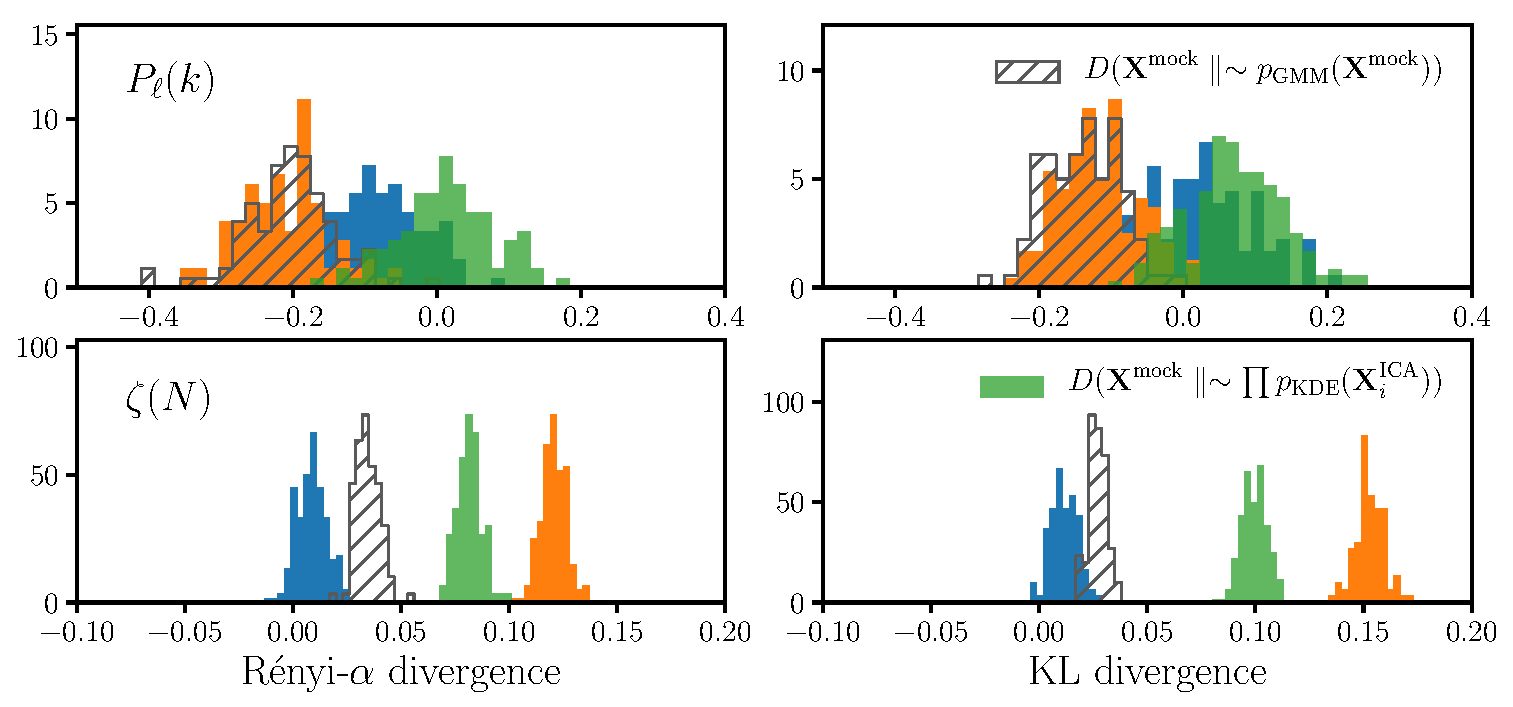
\includegraphics[width=0.9\textwidth]{figs/kNNdiverg_nonGauss.pdf}
\caption{R\'enyi-$\alpha$ and KL divergence}
\label{fig:div_nongauss}
\end{center}
\end{figure}

%%%%%%%%%%%%%%%%%%%%%%%%%%%%%%%%%%%%%%%%%%%%%%%%%%%%%%%%%%%%%%%
% Acknowledgements
%%%%%%%%%%%%%%%%%%%%%%%%%%%%%%%%%%%%%%%%%%%%%%%%%%%%%%%%%%%%%%%
\section*{Acknowledgements}
It's a pleasure to thank 
    Simone~Ferraro,
    David~W.~Hogg,
    Emmaneul~Schaan, 
    Roman~Scoccimarro
    Zachary~Slepian

\bibliographystyle{yahapj}
\bibliography{nongausslike}
\end{document}
